% Created 2020-06-29 Mon 11:46
% Intended LaTeX compiler: pdflatex
\documentclass[presentation]{beamer}
\usepackage[utf8]{inputenc}
\usepackage[T1]{fontenc}
\usepackage{graphicx}
\usepackage{grffile}
\usepackage{longtable}
\usepackage{wrapfig}
\usepackage{rotating}
\usepackage[normalem]{ulem}
\usepackage{amsmath}
\usepackage{textcomp}
\usepackage{amssymb}
\usepackage{capt-of}
\usepackage{hyperref}
\usepackage{minted}
\usepackage[utf8]{inputenc}
\usepackage{color}
\usetheme[height=7mm]{Rochester}
\setbeamertemplate{footline}[frame number]
\usecolortheme[accent=red, light]{solarized}
\setbeamercolor{frametitle}{bg=solarizedRebase02,fg=solarizedAccent}
\setbeamercolor{author in head/foot}{bg=solarizedRebase02,fg=solarizedRebase01}
\setbeamercolor{title in head/foot}{bg=solarizedRebase02,fg=solarizedRebase01}
\setbeamercolor{block title}{bg=solarizedRebase0,fg=solarizedRebase02}
\setbeamercolor{block body}{bg=solarizedRebase02,fg=solarizedRebase0}
\setbeamercolor{item}{bg=solarizedRebase02,fg=solarizedAccent}
\beamertemplatenavigationsymbolsempty
\usemintedstyle{manni}
\AtBeginSection[]{
\begin{frame}
\vfill
\centering
\begin{beamercolorbox}[sep=8pt,center,shadow=true,rounded=true]{title}
\Huge\insertsectionhead\par%
\end{beamercolorbox}
\vfill
\end{frame}
}
\usetheme{default}
\author{Sebastian Stabinger}
\date{SS2020}
\title{Vererbung}
\hypersetup{
 pdfauthor={Sebastian Stabinger},
 pdftitle={Vererbung},
 pdfkeywords={},
 pdfsubject={},
 pdfcreator={Emacs 26.3 (Org mode 9.1.9)}, 
 pdflang={Ger}}
\begin{document}

\maketitle
\section{Das Problem}
\label{sec:org2b7195e}
\begin{frame}[label={sec:org4088d6e}]{Beispiel}
\begin{itemize}
\item Wir wollen Klassen für verschiedene Elemente eines Spiels
deklarieren (z.B. Spieler, Ladenbesitzer, Objekt, \ldots{})
\item Viele Aspekte dieser Klassen sind gleich oder zumindest ähnlich.
Alle haben eine aktuelle Position und ein Bild das angezeigt werden
soll
\item Ein paar Aspekte sind aber anders. z.B. hat ein Spieler evtl.
Lebenspunkte und kann sich bewegen. Ein Ladenbesitzer hat ein
Inventar das er verkaufen kann und ein Objekt kann passierbar sein
oder nicht
\item Mit unserem aktuellen Wissen müssten wir die gemeinsamen
Eigenschaften in der Spieler-, Ladenbesitzer- und Objekt-Klasse
manuell wiederholen.
\end{itemize}
\end{frame}
\begin{frame}[fragile,label={sec:org224795d}]{Beispiel Code --- Spieler}
 \begin{minted}[fontsize=\scriptsize,numberblanklines=false]{c++}
class Player {
private:
  string _image;
  int _xpos, _ypos, _health;

public:
  Player(int xpos, int ypos, int health, string image) {
    _xpos = xpos;
    _ypos = ypos;
    _image = image;
    _health = health;
  }

  void move_up() { ypos--; }
  void move_down() { ypos++; }
  void move_left() { xpos--; }
  void move_right() { xpos++; }

  bool isdead() { return health <= 0; }
  void draw() { draw_img(_image, _xpos * 16, _ypos * 16); }
};
\end{minted}
\end{frame}
\begin{frame}[fragile,label={sec:org69592f9}]{Beispiel Code --- Ladenbesitzer}
 \begin{minted}[fontsize=\scriptsize,numberblanklines=false]{c++}
class Shopkeep {
private:
  string _image;
  int _xpos, _ypos;
  vector<string> _inventory;

public:
  Shopkeep(int xpos, int ypos, string image, vector<string> inventory) {
    _xpos = xpos;
    _ypos = ypos;
    _image = image;
    _inventory = inventory;
  }

  vector<string> get_inventory() { return _inventory; }

  void draw() { draw_img(_image, _xpos * 16, _ypos * 16); }
};
\end{minted}
\end{frame}
\begin{frame}[fragile,label={sec:org720f8b8}]{Beispiel Code --- Objekt}
 \begin{minted}[fontsize=\scriptsize,numberblanklines=false]{c++}
class Object {
private:
  int _xpos, _ypos;
  string _image;
  bool _solid;

public:
  Object(int xpos, int ypos, string image, bool solid) {
    _xpos = xpos;
    _ypos = ypos;
    _image = image;
    _solid = solid;
  }

  bool issolid() { return solid; }
  void draw() { draw_img(_image, _xpos * 16, _ypos * 16); }
};
\end{minted}
\end{frame}
\section{Die Lösung --- Vererbung}
\label{sec:orgc9676a6}
\begin{frame}[fragile,label={sec:orgb6dae2b}]{Vererbung}
 \begin{itemize}
\item Mittels Vererbung kann eine Klasse (die \alert{abgeleitete Klasse})
Variablen und Memberfunktionen einer anderen Klasse (der
\alert{Basisklasse}) erben und somit verwenden.
\item Wir erweitern und/oder ändern also die Funktionalität einer bereits
existierenden Klasse (die \alert{Basisklasse}) und geben dieser geänderten
Klasse (die \alert{abgeleitete Klasse}) einen neuen Namen.
\item Wir sagen \alert{die abgeleitete Klasse erweitert die Basisklasse}
\end{itemize}
\begin{block}{Syntax}
\begin{minted}[fontsize=\scriptsize,numberblanklines=false]{c++}
class AbgeleiteteKlasse : public Basisklasse {
  // ... Definition der abgeleiteten Klasse
}
\end{minted}
\end{block}
\begin{itemize}
\item \alert{Achtung}: Die abgeleitete Klasse hat nur Zugriff auf Variablen und
Memberfunktionen der Basisklasse welche {\color{solarizedYellow}\texttt{public} }sind!
\end{itemize}
\end{frame}
\begin{frame}[fragile,label={sec:org8eb3b19}]{Vererbung --- Kurzes Beispiel}
 \begin{minted}[fontsize=\scriptsize,numberblanklines=false]{c++}
#include <iostream>
using namespace std;

class HelloWorldBasis {
public:
  int num1 = 42;
  void print1() { cout << "Hallo: Basisklasse " << num1 << endl; }
};

class HelloWorldAbgeleitet : public HelloWorldBasis {
public:
  int num2 = 23;
  void print2() { cout << "Hallo: Abgeleitete Klasse " << num1 << endl; }
};

int main() {
  HelloWorldBasis w1;
  w1.print1(); // Output: Hallo : Basisklasse 42
  HelloWorldAbgeleitet w2;
  w2.print2(); // Output: Hallo : Abgeleitete Klasse 42
  // Die Funktion print1 ist auch in der abgeleiteten Klasse
  w2.print1(); // Output: Hallo : Basisklasse 42
  cout << "num = " << w2.num1 << endl;  // 42
  cout << "num2 = " << w2.num2 << endl; // 23
}
\end{minted}
\end{frame}
\begin{frame}[label={sec:orgae86f3e}]{Vererbung --- Kurzes Beispiel}
Grafisch kann man sich die Vererbung folgendermaßen vorstellen (Die
Basisklasse ist in die abgeleitete Klasse eingebettet):
\begin{center}\begin{center}
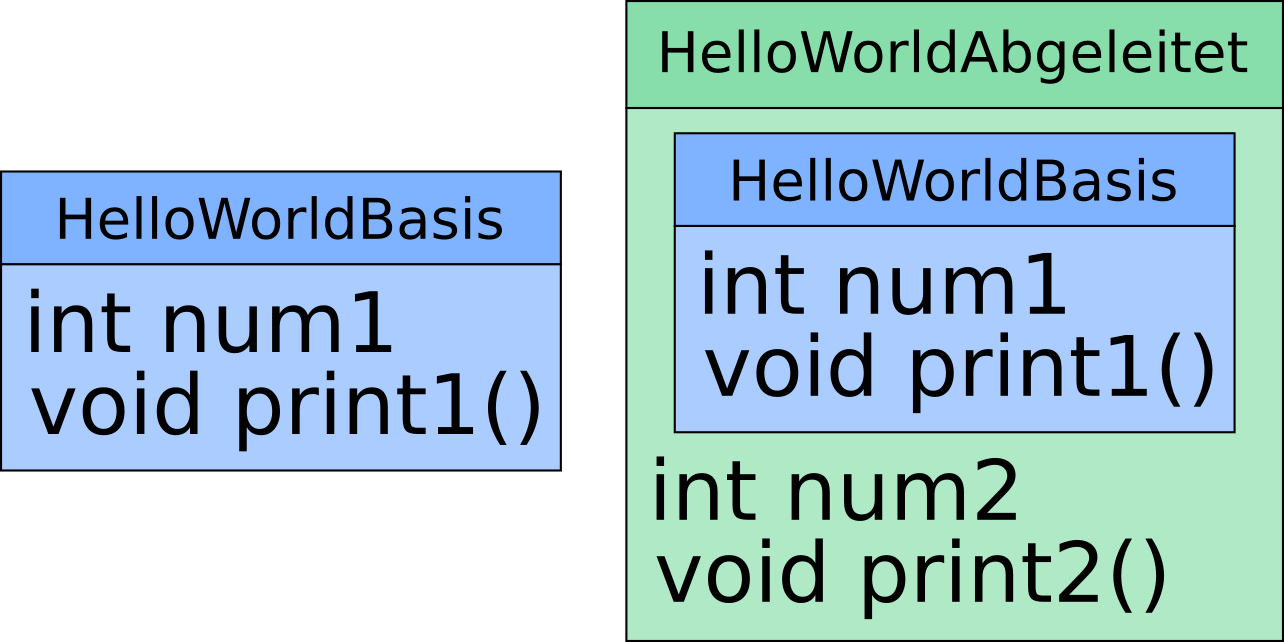
\includegraphics[width=.9\linewidth]{imgs/helloworldbasisabgeleitet.png}
\end{center}\end{center}
\end{frame}
\section{Überladen von Funktionen}
\label{sec:org3bb0f33}
\begin{frame}[fragile,label={sec:org3cf9603}]{Funktionsweise}
 Wir können eine Funktion der Basisklasse in der abgeleiteten Klasse
überschreiben indem wir sie gleich benennen.
\begin{minted}[fontsize=\scriptsize,numberblanklines=false]{c++}
#include <iostream>
using namespace std;

class HelloWorldBasis {
public:
  int num1 = 42;
  void print() { cout << "Hallo: Basisklasse " << num1 << endl; }
};

class HelloWorldAbgeleitet : public HelloWorldBasis {
public:
  int num2 = 23;
  void print() { cout << "Hallo: Abgeleitete Klasse " << num1 << endl; }
};

int main() {
  HelloWorldBasis w1;
  w1.print(); // Output: Hallo : Basisklasse 42
  HelloWorldAbgeleitet w2;
  w2.print();  // Output: Hallo : Abgeleitete Klasse 42
  cout << "num = " << w2.num1 << endl;  // 42
  cout << "num2 = " << w2.num2 << endl; // 23
}
\end{minted}
\end{frame}
\begin{frame}[label={sec:orgc3ea7d7}]{Überladen von Funktionen}
\begin{center}\begin{center}
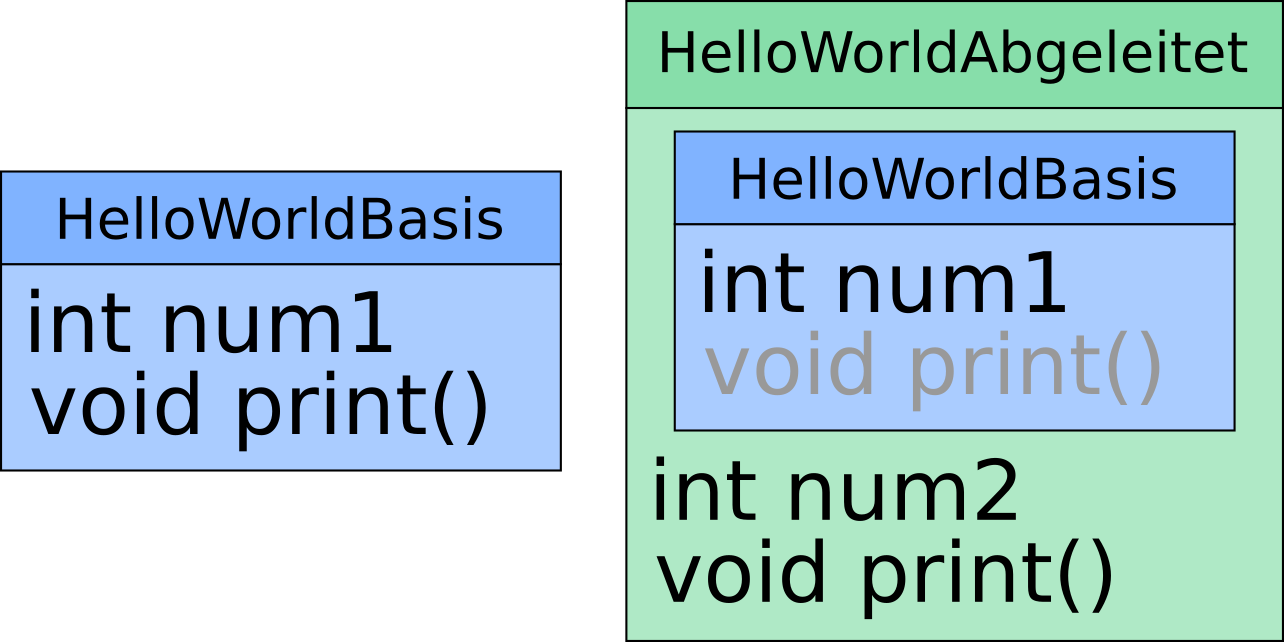
\includegraphics[width=.9\linewidth]{imgs/overload.png}
\end{center}\end{center}
\begin{itemize}
\item Das System sucht sozusagen von \alert{Außen nach Innen} und führt die
erste Funktion aus welche hinsichtlich Namen und Parametern passt
\end{itemize}
\end{frame}
\begin{frame}[fragile,label={sec:org4d20921}]{Verwendung überschriebener Funktionen}
 \begin{block}{Problem}
\begin{itemize}
\item Wir haben in {\color{solarizedYellow}\texttt{HelloWorldAbgeleitet} }das vererbte {\color{solarizedYellow}\texttt{print} }von
{\color{solarizedYellow}\texttt{HelloWorldBasis} }überschrieben
\item Wir wollen irgendwo in {\color{solarizedYellow}\texttt{HelloWorldAbgeleitet} }trotzdem das {\color{solarizedYellow}\texttt{print}}
von {\color{solarizedYellow}\texttt{HelloWorldBasis} }aufrufen
\item Was z.B. häufig vorkommt: Wir erweitern eine Funktion der
Basisklasse indem wir sie überschreiben. In der neuen Funktion rufen
wir die überschiebene Funktion der Basisklasse auf.
\end{itemize}
\end{block}
\begin{block}{Lösung}
\begin{itemize}
\item \alert{Wir können auf die Basisklasse wie auf einen Namespace zugreifen.}
\item Bsp. {\color{solarizedYellow}\texttt{HelloWorldBasis::print()}}
\end{itemize}
\end{block}
\end{frame}
\begin{frame}[fragile,label={sec:orgd4d7f39}]{Verwendung überschriebener Funktionen}
 \begin{minted}[fontsize=\scriptsize,numberblanklines=false]{c++}
#include <iostream>
using namespace std;

class HelloWorldBasis {
public:
  int num1 = 42;
  void print() { cout << "Hallo: Basisklasse " << num1 << endl; }
};

class HelloWorldAbgeleitet : public HelloWorldBasis {
public:
  int num2 = 23;
  void print() {
    HelloWorldBasis::print();
    cout << "Hallo: Abgeleitete Klasse " << num1 << endl;
  }
};

int main() {
  HelloWorldAbgeleitet w2;
  w2.print();
  // Output:
  // Hallo : Basisklasse 42
  // Hallo : Abgeleitete Klasse 42
}
\end{minted}
\end{frame}
\section{Konstruktoren und Vererbung}
\label{sec:org3127b60}
\begin{frame}[fragile,label={sec:org699fb72}]{Standardkonstruktoren}
 Der Standardkonstruktor einer Basisklasse wird automatisch aufgerufen
wenn die abgeleiteten Klasse erzeugt wird.
\begin{minted}[fontsize=\scriptsize,numberblanklines=false]{c++}
#include <iostream>

class C1 {
public:
  int i;
  C1() { i = 23; }
};

class C2 : public C1 {
public:
  int j;
  C2() { j = 42; }
};

int main() {
  C2 c;
  std::cout << c.i << " " << c.j << std::endl; // Output: 23 42
}
\end{minted}
\end{frame}
\begin{frame}[fragile,label={sec:org16c2e6b}]{Konstruktoren mit Parametern}
 Ein Konstruktor der Basisklasse welcher Parameter erwartet \alert{muss
explizit aufgerufen werden}. Dies geschieht durch Anhängen mittels {\color{solarizedYellow}\texttt{:}}
an den Konstruktor.
\begin{exampleblock}{Syntax --- Beispiel}
\begin{minted}[fontsize=\scriptsize,numberblanklines=false]{c++}
class C1 {
public:
  int a;
  C1(int pa) { a = 2 * pa; }
};

class C2 : public C1 {
public:
  C2(int i) : C1(3 * i) { a = a + 10; }
};

int main() {
  C2 c(4); // c.a == 34 [(2*(3*4))+10]
  cout << c.a << endl;
}
\end{minted}
\end{exampleblock}
\end{frame}
\section{Ein größeres Beispiel}
\label{sec:orgbd756be}
\begin{frame}[fragile,label={sec:org12396fe}]{Code Beispiel --- Ein Ding}
 \begin{minted}[fontsize=\scriptsize,numberblanklines=false]{c++}
class Thing {
private:
  int _xpos, _ypos;
  string _image;

public:
  Thing(int xpos, int ypos, string image) {
    _xpos = xpos;
    _ypos = ypos;
    _image = image;
  }

  int get_xpos() { return _xpos; }
  int get_ypos() { return _ypos; }
  void set_xpos(int x) { _xpos = x; }
  void set_ypos(int y) { _ypos = y; }

  void draw() { draw_image(_image, _xpos * 16, _ypos * 16); }
};
\end{minted}
\end{frame}
\begin{frame}[fragile,label={sec:orgeccb450}]{Code Beispiel --- Spieler}
 \begin{minted}[fontsize=\scriptsize,numberblanklines=false]{c++}
class Player : public Thing {
private:
  int _health;

public:
  Player(int xpos, int ypos, int health, string image)
      : Thing(xpos, ypos, image) {
    _health = health;
  }

  void move_up() { set_ypos(get_ypos() - 1); }
  void move_down() { set_ypos(get_ypos() + 1); }
  void move_left() { set_xpos(get_xpos() - 1); }
  void move_right() { set_xpos(get_xpos() - 1); }

  void draw() { // Erweitere draw Funktion von Thing
    Thing::draw();
    // Zeichne Gesundheitsanzeige ...
  }
};
\end{minted}
\end{frame}
\begin{frame}[label={sec:orgf8bd58e}]{Graphische Visualisierung --- Thing - Player}
\begin{center}\begin{center}
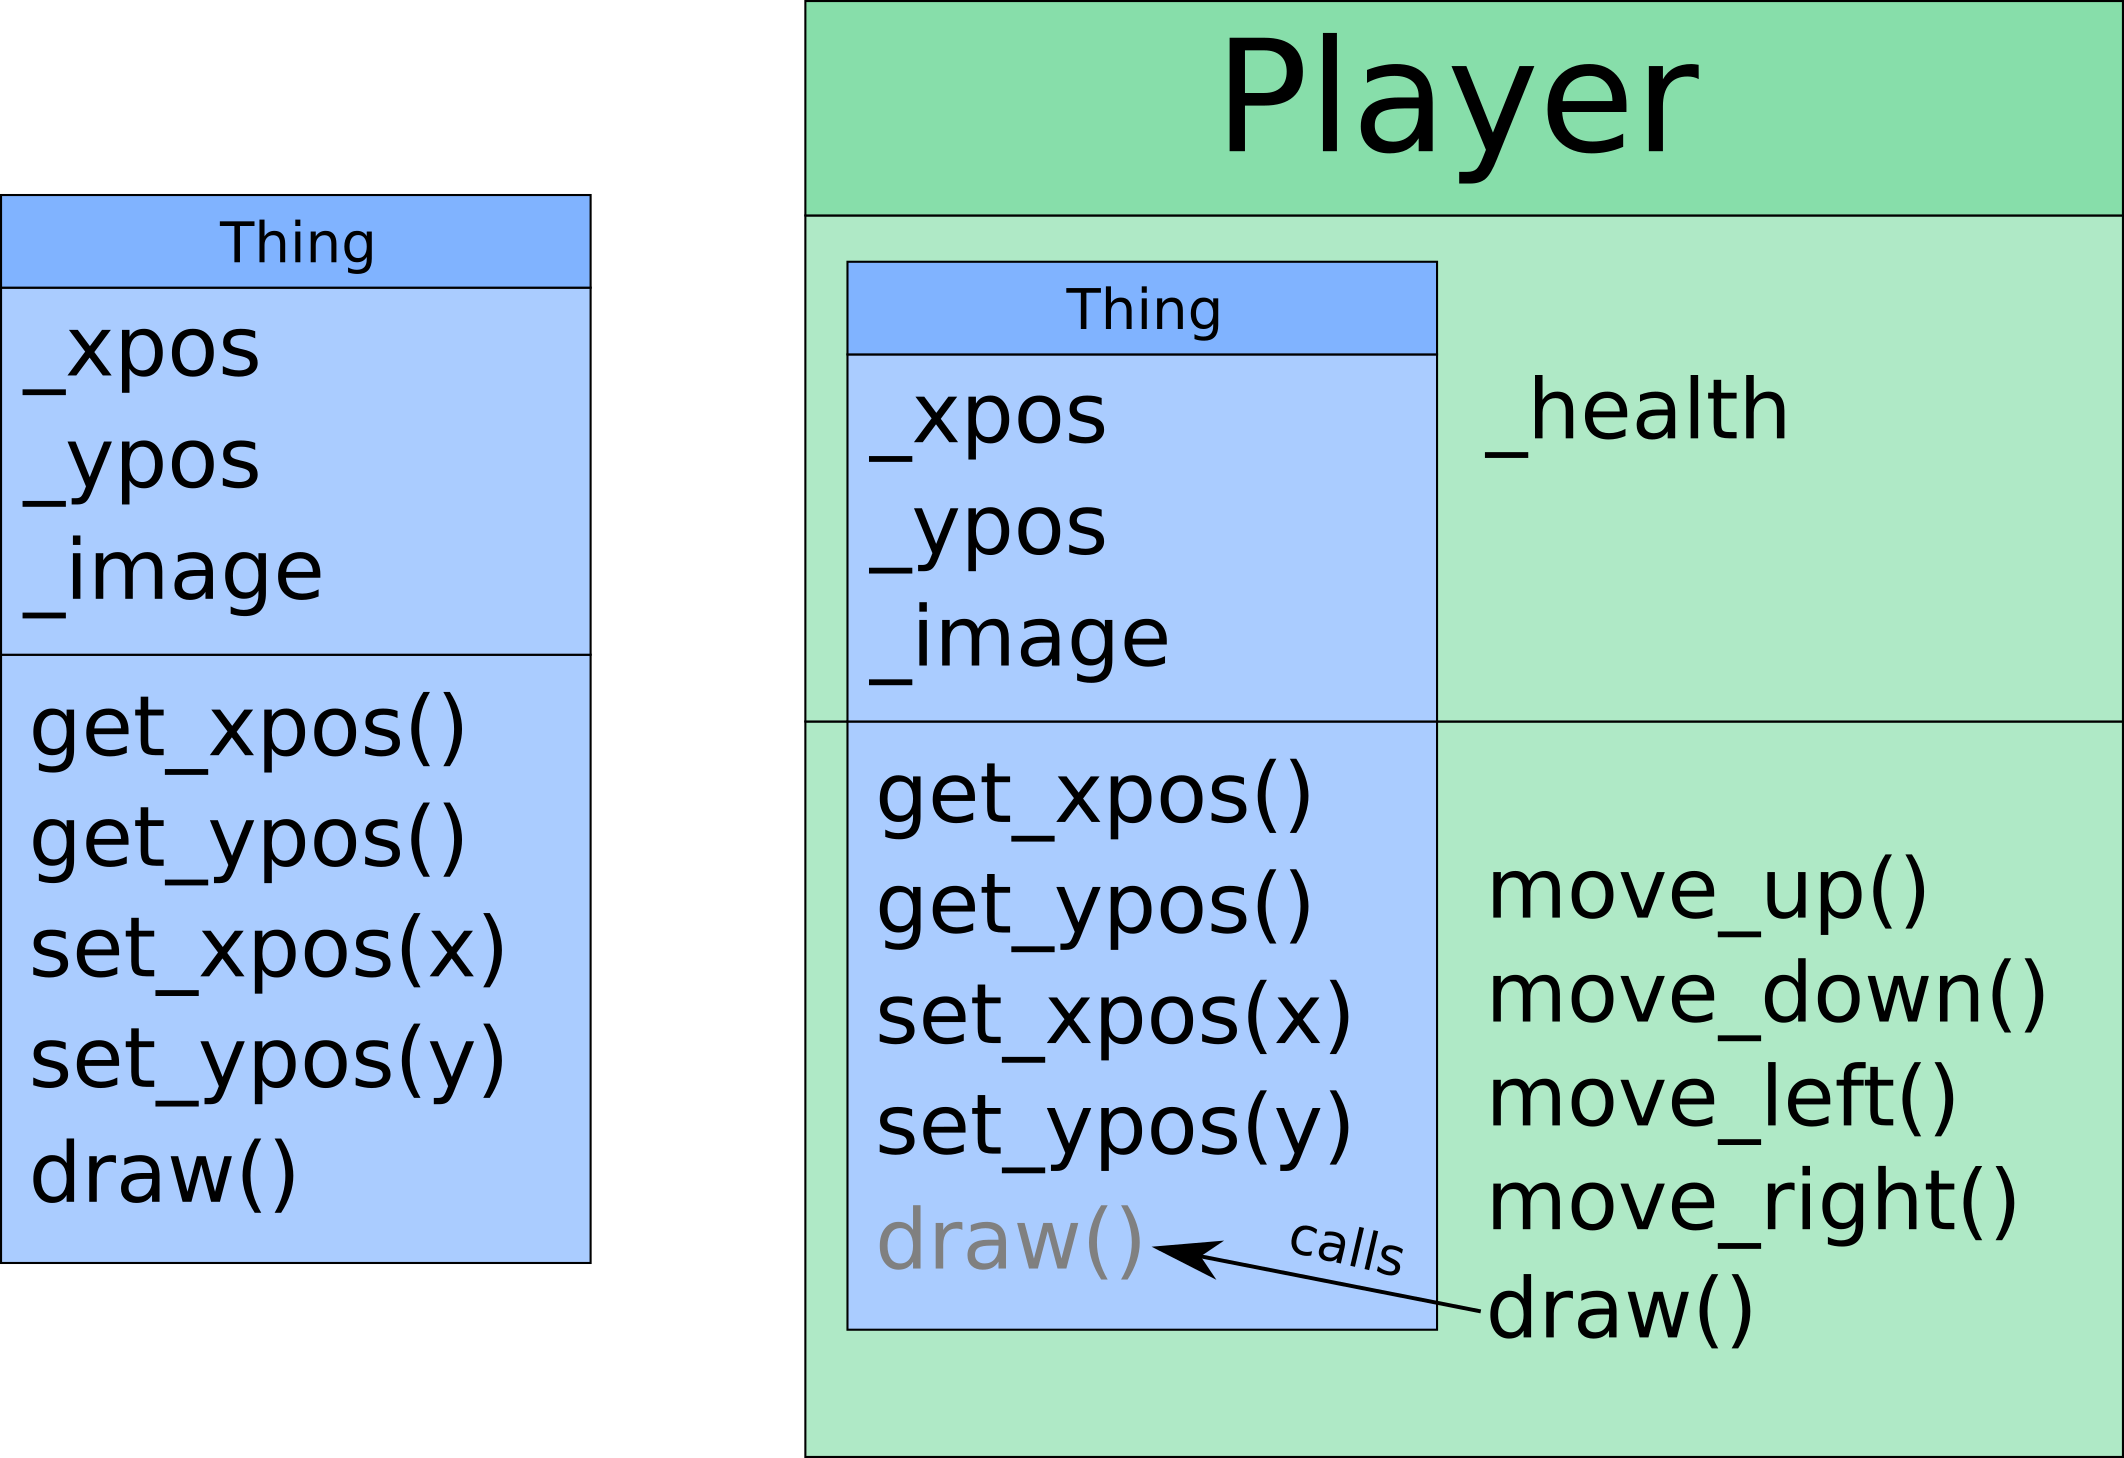
\includegraphics[width=.9\linewidth]{imgs/thingplayer.png}
\end{center}\end{center}
\end{frame}
\begin{frame}[fragile,label={sec:orgdf1d39a}]{Code Beispiel --- Ladenbesitzer}
 \begin{minted}[fontsize=\scriptsize,numberblanklines=false]{c++}
class Shopkeep : public Thing {
private:
  vector<string> _inventory;

public:
  Shopkeep(int xpos, int ypos, string image, vector<string> inventory)
      : Thing(xpos, ypos, image) {
    _inventory = inventory;
  }

  vector<string> get_inventory() { return _inventory; }
};
\end{minted}
\end{frame}
\begin{frame}[fragile,label={sec:org915f723}]{Code Beispiel --- Objekt}
 \begin{minted}[fontsize=\scriptsize,numberblanklines=false]{c++}
class Object : public Thing {
private:
  bool _solid;

public:
  Object(int xpos, int ypos, string image, bool solid)
      : Thing(xpos, ypos, image) {
    _solid = solid;
  }

  bool issolid() { return _solid; }
};
\end{minted}
\end{frame}
\section{Kontrolle der Sichtbarkeit}
\label{sec:orgdd3ead4}
\begin{frame}[fragile,label={sec:orge3d7d30}]{Das Problem}
 \begin{itemize}
\item Wir haben bereits gelernt: Die abgeleitete Klasse hat Zugriff auf
alle Elemente der Basisklasse welche {\color{solarizedYellow}\texttt{public} }sind. Auf die
{\color{solarizedYellow}\texttt{private} }Elemente hat sie \alert{keinen} Zugriff.
\item Wir wollen aber häufig in der abgeleiteten Klasse direkt auf
Elemente der Basisklasse zugreifen welche von außerhalb nicht
sichtbar sind.
\end{itemize}
\begin{exampleblock}{Beispiel}
\begin{minted}[fontsize=\scriptsize,numberblanklines=false]{c++}
class C1 {
private:
  int secret;
};

class C2 : public C1 {
public:
  void change_secret(int newsecret) { secret = newsecret; }
  // Error!! Kein Zugriff auf secret
};
\end{minted}
Wir könnten {\color{solarizedYellow}\texttt{secret} }in den {\color{solarizedYellow}\texttt{public} }Bereich schieben, aber dann kann
jeder darauf zugreifen \ldots{}
\end{exampleblock}
\end{frame}
\begin{frame}[fragile,label={sec:org83f4000}]{Die Lösung: protected}
 \begin{itemize}
\item Um dieses Problem zu lösen gibt es einen dritten
Sichtbarkeitsbereich innerhalb einer Klasse namens {\color{solarizedYellow}\texttt{protected}}
\item Er verhält sich von Außerhalb so wie {\color{solarizedYellow}\texttt{private}}, aber eine
abgeleitete Klasse kann direkt darauf zugreifen.
\end{itemize}
\begin{exampleblock}{Beispiel}
\begin{minted}[fontsize=\scriptsize,numberblanklines=false]{c++}
class C1 {
protected:
  int secret;
};

class C2 : public C1 {
public:
  void change_secret(int newsecret) { secret = newsecret; }
};

int main() {
  C2 c;
  c.change_secret(42); // Alles OK
  c.secret;            // Error!! Kein Zugriff auf secret
}

\end{minted}
\end{exampleblock}
\end{frame}
\section{Übungen}
\label{sec:org4057eb3}
\begin{frame}[label={sec:orgba4973f}]{Gemeinsame Übung}
Wir schreiben die beim letzten Termin entwickelte Version des Spiels
so um, dass es eine \alert{Spieler- und eine Monsterklasse} gibt.
\begin{itemize}
\item Der Spieler bekommt eine Gesundheitsanzeige
\item Die Monster verschwinden wie gehabt nach einer gewissen Zeit, wir
lösen das dieses mal aber in der Monsterklasse selbst
\end{itemize}
\end{frame}
\end{document}